\section{Water Models}\label{sec:water_models}

% Navier stokes, Different level of water depth, Spatial, Spectral domain,
% eulerian, lagrangian frameworks, talk about their visual accuracy, SLProject,
% 0 a.d.


\subsection{Navier Stokes Equations}\label{subsec:navier_stokes}
\subsection{Spatial Domain}\label{subsec:spatial_domain}
\subsection{Spectral Domain}\label{subsec:spectral_domain}
\subsection{Methods Used in Industry Productions}\label{subsec:methods_industry}

% FFT, Projected Grid, LOD,

\subsection{Candidate Applications for Embedding}\label{subsec:candidate_apps}

% SLProject, 0 a.d.

We now present two candidate applications which need a real-time water model:
\textit{SLProject} and \textit{0 A.D.}\footnote{Although both have already one,
in the former application the model doesn't work and in the latter it is
outdated.}.

\subsubsection{SLProject}



\subsubsection{0 A.D.}

% Talk about the history of the project, what it is, how it is maintained,
% open source, game engine, the tickets and contacts with the devs.

\textit{0 A.D.} is a real-time strategy game representing the 500 B.C to 500 A.D
era. It is developed by Wildfire Games, an independent game development studio.
The game is free, open source\footnote{Licensed under the GNU-GPL and CC BY-SA
license.} and runs on Windows, MacOS and Linux.

The development of the game began in 2000 when three modding groups whished to
create a free game engine. Up until 2009 the source code was accessible only to
members of Wildfire Games. Anyone interested in participating could make an
application and pass an interview. However, due to the fading interest of a
mod\footnote{Shorthand for the term \textit{modification}} which used 0 A.D.'s
game engine and the lack of programmers, they opened up the code in July 2009.
From then on many contributions have been made, notably one redesigning entirely
the code base, making new contributions easier. As of today the project is still
actively maintained, with the latest alpha-release (number 22 code named
``Venustas'') dating from July 26,
2017~\autocite{wildfire0adproject,wildfire0adstory}.

The game engine, Pyrogenesis, is heavily oriented towards modding. The core
engine is coded in C++ and Javascript is used for the game's logic, like the
artificial intelligence or the random generation of maps. This means that when
\textit{0 A.D.} is run the game engine is started with a given mod. A mod
contains all the graphical elements, 3D models, sound, shaders, scenarios, map
generators and artificial intelligence.

The documentation for developers provides good build instructions, coding
conventions and codebase descriptions. Unfortunately we found that it is
difficult for a newcomer to understand the game engine architecture. It is less
documented and scattered accross multiple pages which are sometimes outadated.
The Doxygen documentation is minimalistic and unlike the one from
\textit{SLProject}, does not help to understand the architecture.

The current water implementation has been created in 2006 by a student form the
University of Waterloo, Canada, as a course project~\autocite{zaharia2006cs}.
Over the years it has been slightly modified and optimized but appears visually
outdated (see~\autoref{fig:0ad_water}) compared to the one used in
commercial RTS games like Anno 1800 or Age of Empires~3. There is an open
ticket, \#48 ``Advanced Water Rendering'', which was opened twelve years ago and
modified three years ago but still not closed.  We have contacted the developers
and they would gladly appreciate a contribution that would close the issue.

%\missingfigure{screenshot of 0ad water}

\begin{figure}[t!]
    \centering
    \begin{subfigure}[t]{\textwidth}
        \centering
        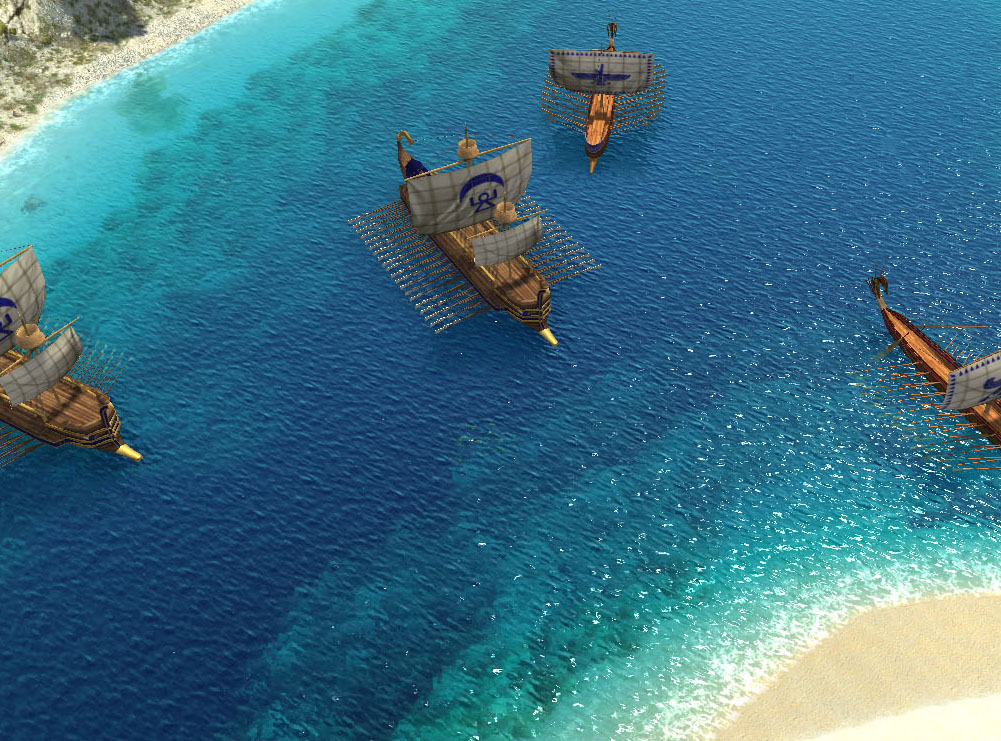
\includegraphics[height=5cm]{figures/0ad_water-specular.jpg}
        \subcaption{Close view of the water.}\label{subfig:0ad_water_close}
    \end{subfigure}\\%
    %  
    \begin{subfigure}[t]{\textwidth}
        \centering
        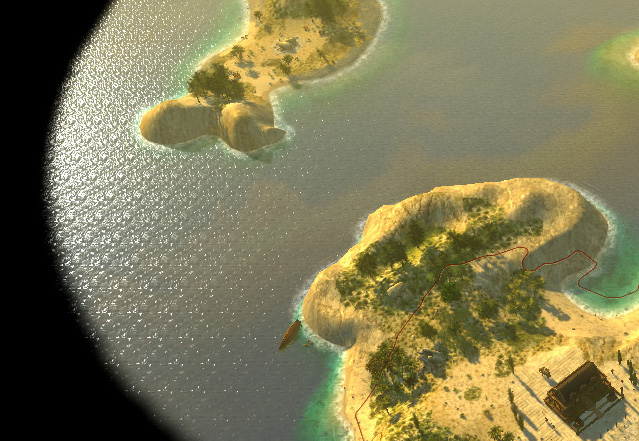
\includegraphics[height=5cm]{figures/0ad_cycladic_arcgipelago_6.jpg}
        \subcaption{Zoomed out view.}\label{subfig:0ad_water_far}
    \end{subfigure}
    \caption{\textit{0 A.D.}'s water rendering. Notice on the lower left part
        of~\autoref{subfig:0ad_water_close} the repetition of the waves.
        In~\autoref{subfig:0ad_water_far} it is even more apparent (source:
        \url{play0ad.com}).}\label{fig:0ad_water}
\end{figure}
